\documentclass[a4paper, 12pt]{article}
\usepackage[utf8]{inputenc}

\title{História e Futuro da Computação (IF690)}
\author{Williams Douglas}
\date{Outubro de 2019}
\usepackage[onehalfspacing]{setspace}
\usepackage{natbib}
\usepackage{graphicx,indentfirst}
\usepackage[lmargin=3cm, tmargin=3cm, rmargin=2cm, bmargin=2]{geometry}

\begin{document}

\maketitle


\emph{"Quando eu estava na escola, o computador era uma coisa muito assustadora. As pessoas falavam em desafiar aquela máquina do mal que estava sempre fazendo contas que não pareciam corretas. E ninguém pensou naquilo como uma ferramenta poderosa."}

Bill Gates em palestra, no ano de 2004.\cite{billgates}

\section{Introdução}
A disciplina História e Futuro da Computação, oferecida pelo Cin, busca mostrar ao aluno toda a evolução dos conceitos e marcos fundamentais da computação, apresentando não só o histórico, mas também grandes ideias e metáforas da computação. Além de aprensetar  novas tendências tecnológicas como o conceito de computação quântica e biológica.



\begin{figure}[h!]
\centering
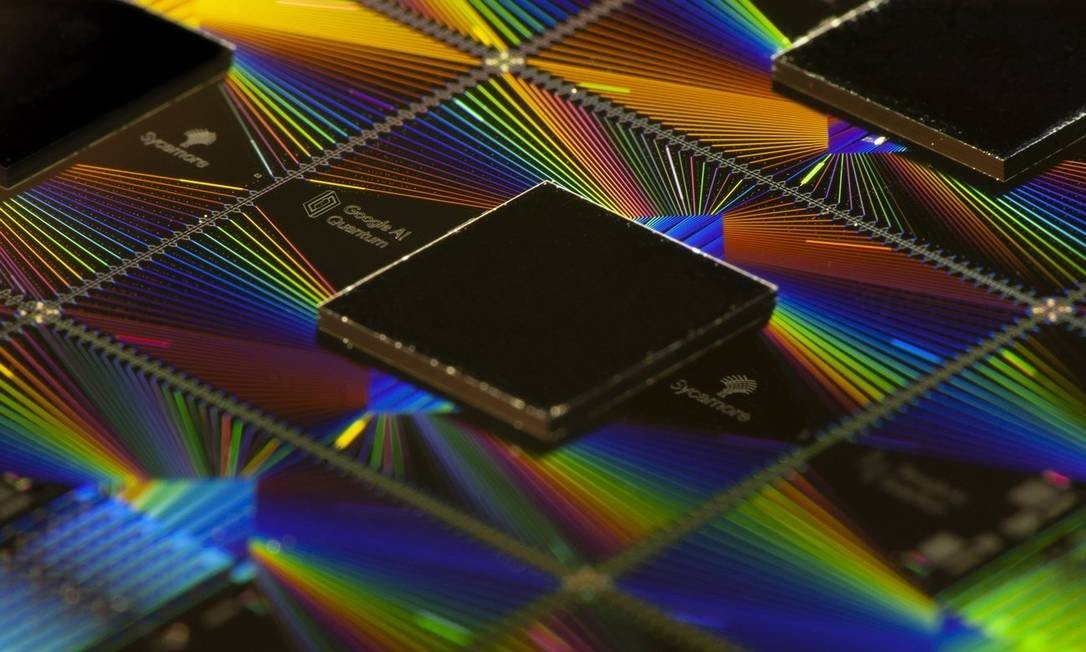
\includegraphics[scale=0.2]{chipquantico.jpg}
\caption{Chip quântico Sycamore desenvolvido pela Google, a qual afirma ter atigindo a "Supremacia quântica", dando assim, um passo importantíssimo no futuro da computação.\cite{oglobo2019supremacia}}
\label{fig:chipquantico.jpg}
\end{figure}

\section{Relevância}
É de enorme importância para o aluno conhecer a história do desenvolvimento tecnológico, como os primeiros computadores e sistemas eletrôncos que nos trouxeram ao ponto atual de desenvolvimento, criando relações com o futuro da computação, vendo novos e antigos paradigmas computacionais.\newpage Essa disciplina permeia de forma histórica vários outros tópicos abordados de forma técnica por outras disciplinas do curso de Ciência da Computação, como disciplinas de Software, Hardware e Comunicação.
\begin{figure}[h!]
\centering
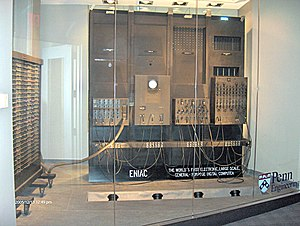
\includegraphics[scale=0.8]{eniac.jpg}
\caption{ENIAC, primeiro computador digital eletrônico de grande escala, lançado em 1946.\cite{eniac}}
\label{fig:eniac.jpg}
\end{figure}
\section{Relação com outras disciplinas}
A disciplina História e Futuro da Computação possui como pré-requisito a disciplina de Introdução a Computação(IF668), não sendo pré-requisito de nenhuma outra.


\bibliographystyle{plain}
\bibliography{wdjs}
\end{document}
